%*******************************************************************************
%****************************** Second Chapter *********************************
%*******************************************************************************

\chapter{Experimental Methods}

\section{Transmission Electron Microscopy}
\label{TEM}
A typical transmission electron microscope  \nomenclature[z-TEM]{TEM}{Transmission Electron Microscope} (TEM) consists of a high voltage (typically 100-400kV) electron gun under extremely high vacuum conditions within a column. The beam of electrons generated by this gun passes through a set of lenses which focus or deflect the beam before it is incident on the sample under examination. If this sample is thin enough to be electron transparent, the electrons passing through it and scattering elastically or inelastically can be collected using a subsequent set of lenses, apertures and a detector. A simplified schematic of a TEM illumination system is shown in Fig.\ref{2.11}:

\begin{figure}[!ht]
	\centering
	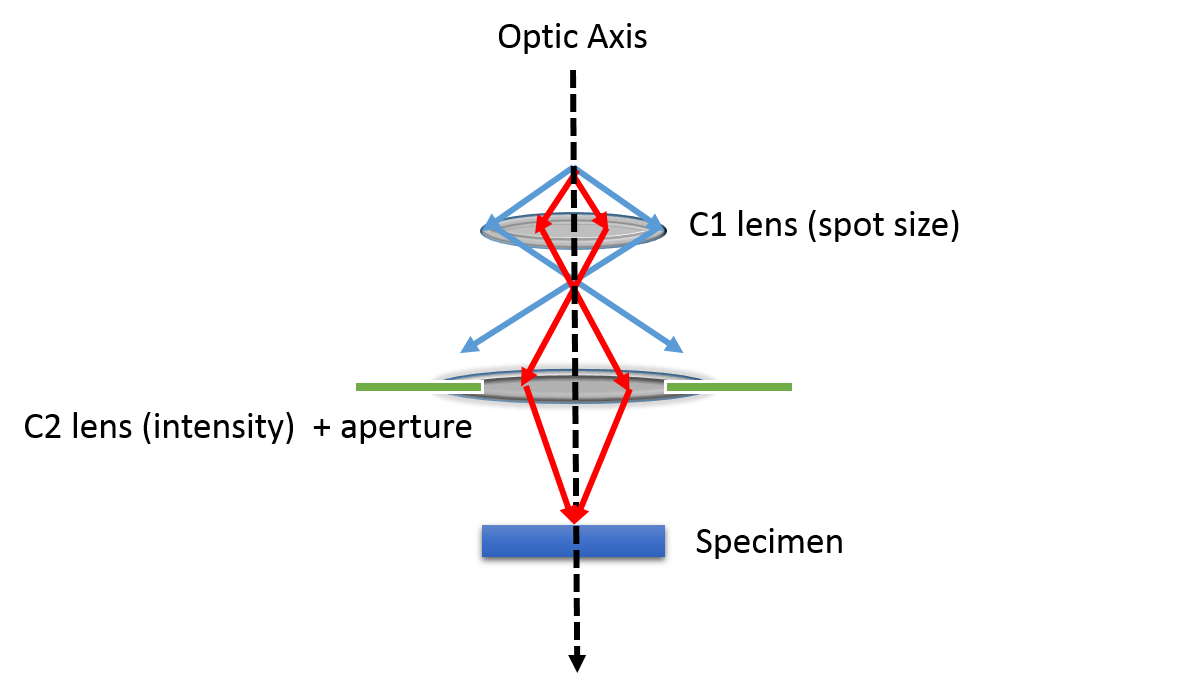
\includegraphics[width=0.9\textwidth]{Figs/Ch2/illum.png}
	\caption[h] {Simplified TEM illumination system.}
	\label{2.11}
\end{figure}

\FloatBarrier 

It important to consider the range of electron-specimen interactions which occur as the high energy electron beam impact the sample. These interactions can be divided into two main categories according to whether the electron kinetic energy is either conserved or not during the interaction, known as elastic or inelastic respectively. Different elastic and inelastic signals produced by the electron-specimen interaction are illustrated in Fig.\ref{2.12}.

\begin{figure}[h]
	\begin{subfigure}[t]{0.5\textwidth}
		\centering
		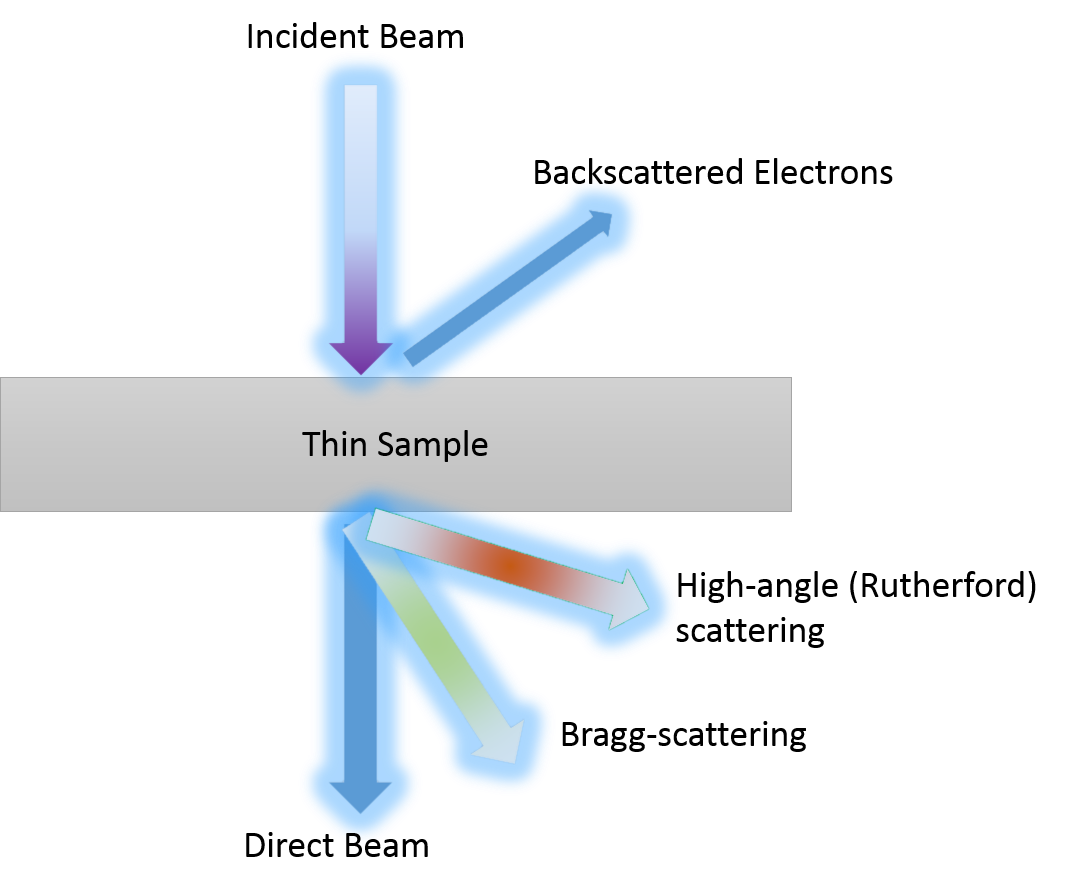
\includegraphics[width = 1\textwidth]{Figs/Ch2/elastic.png}
		\caption{}
	\end{subfigure}%
	\hspace*{1cm}
	~	
	\begin{subfigure}[t]{0.5\textwidth}
		\centering
		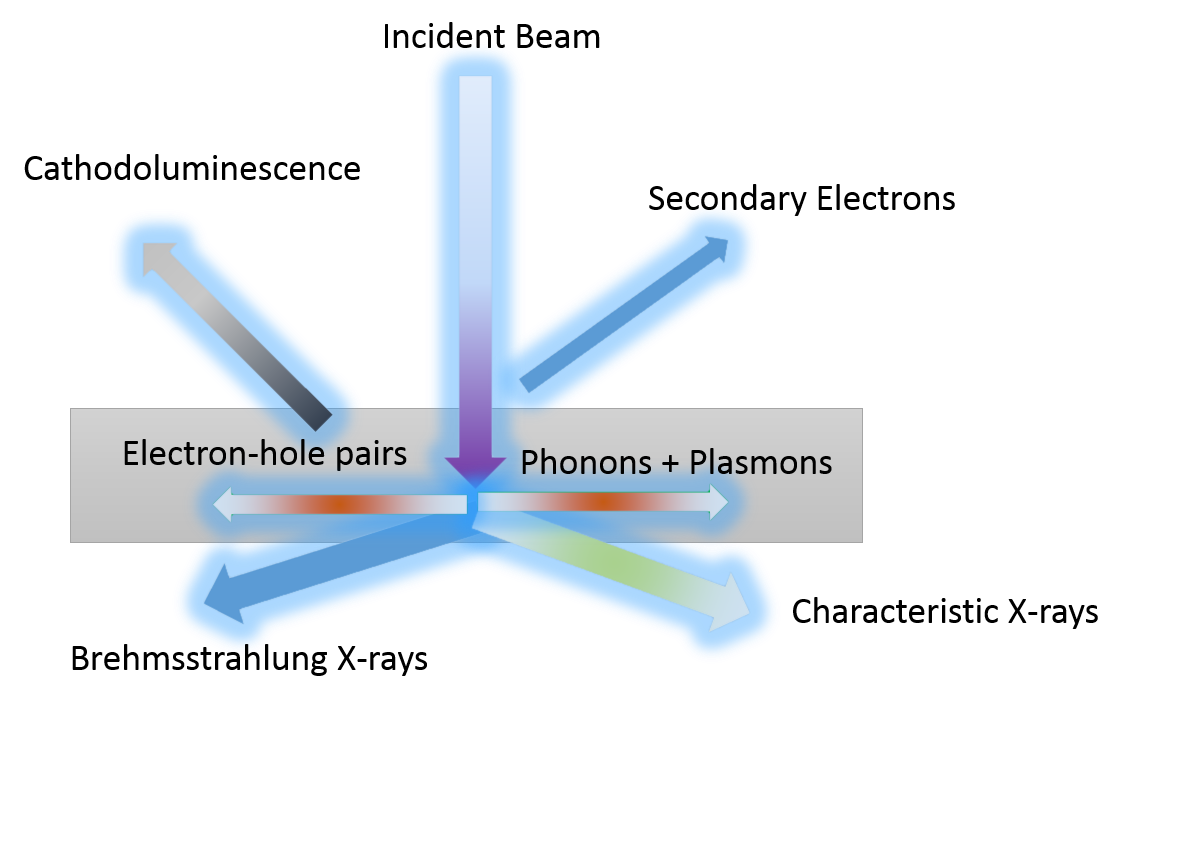
\includegraphics[width=1\textwidth]{Figs/Ch2/inelastic.png}
		\caption{}
	\end{subfigure}
	\caption {a) Elastic and b) inelastic interactions for a high energy electron beam incident on a thin sample. }
	\label{2.12}
\end{figure}
\FloatBarrier 

Fig.\ref{2.12} a) illustrates the importance of sample thickness in TEM. Without a thin specimen, the forward scattered signals such as high-angle and bragg-scattered electrons as well as the direct beam are unavailable.
Given the diversity of scattering interactions  which can occur throughout the sample and contribute to the final signal, different apertures and detectors must be used to extract useful information. The following sections will introduce the different TEM techniques used in this report and their underlying principles. 

\subsection{Conventional Transmission Electron Microscopy} \label{TEMconventional}
\subsubsection{Electron Diffraction}
Electron diffraction is the basis for many TEM techniques as it provides local crystallographic specimen information. The process of diffraction occurs for electrons due to their dual nature as both particles and waves.A beam of electrons can thus be interpreted as a plane wave: the incidence of this plane wave on the specimen results in the scattering of the electrons by atoms through the Coloumb interaction, diffracting the wave in a  manner described by Bragg's law. This is given by Eq. \ref{Bragg}.

\begin{equation}\label{Bragg}
n\lambda = 2d_{hkl}sin\theta_{B}
\end{equation}
where n is an integer, $\lambda$ is the wavelength of the plane wave, $d_{hkl}$ is the crystal plane spacing described by the Miller indices h,k and l and $\theta_{B}$ is the angle between the plane normal and the scattered wave, also known as the Bragg angle.\\
Understanding of the diffraction patterns observed in TEM requires consideration of the reciprocal lattice of the crystal. The reciprocal lattice is defined as the Fourier transform of the crystal lattice, as such the relation of the real-space unit-cell lattice points $\mathbf{a}$, $\mathbf{b}$ and $\mathbf{c}$ to their reciprocal lattice counterparts $\mathbf{a^{*}}$, $\mathbf{b^{*}}$ and $\mathbf{c^{*}}$ can be described as:

\begin{equation}
\mathbf{a^{*}} = \frac{\mathbf{b} \times \mathbf{c}}{V_{c}}, \mathbf{b^{*}} = \frac{\mathbf{c} \times \mathbf{a}}{V_{c}}, \mathbf{c^{*}} = \frac{\mathbf{a} \times \mathbf{b}}{V_{c}}
\end{equation}

where $V_{c}$ is the volume of the unit cell and is given by the relation"

\begin{equation}
V_{c} = \mathbf{a} \cdot \mathbf{b} \times \mathbf{c}
\end{equation}

As such one can define lattice points in reciprocal space which are normal to the plane ($hkil$) in the real lattice as:

\begin{equation}
r^{*} = h\mathbf{a^{*}_{1}} + k\mathbf{a^{*}_{2}} + i\mathbf{a^{*}_{3}} + l\mathbf{c^{*}}
\end{equation}

where $\mathbf{a_{1}}$, $\mathbf{a_{2}}$, $\mathbf{a_{3}}$ and $\mathbf{c}$ are the four hexagonal unit-cell vectors as shown in Fig.\ref{2.13}.

\begin{figure}[!ht]
	\centering
	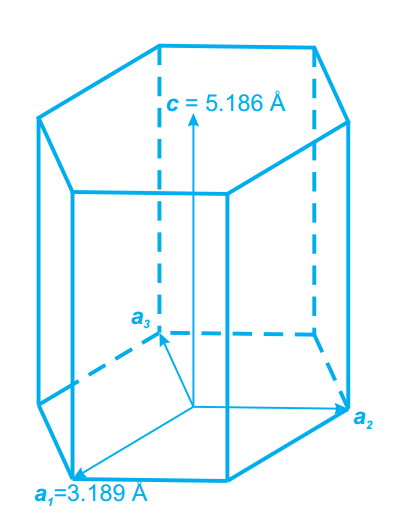
\includegraphics[width=0.3\textwidth]{Figs/Ch2/unitcell.png}
	\caption[h] {Hexagonal GaN lattice in real space with unit-cell vectors defined. Adapted from \cite{Zhang2008}.}
	\label{2.13}
\end{figure}
\FloatBarrier

Considering a beam of electrons of wavelength $\lambda$ incident on a crystal lattice, one can define a sphere in reciprocal space with radius $\frac{1}{\lambda}$ which describes the scattering of the electron beam known as the Ewald sphere. The intersection of the Ewald sphere with lattice points in reciprocal space represent the diffraction spots which can be observed. Typically, the geometry of the TEM specimen results in elongated reciprocal lattice points known as rel-rods. This elongation allows the Ewald sphere to intersect a greater number of 'points', even with slight deviations to the Bragg condition. The scattering vector $\mathbf{K}$ can thus be described as:
\begin{equation}
\mathbf{K} = \mathbf{k_{D}} - \mathbf{k_{I}} = \mathbf{g} + \mathbf{s}
\end{equation}

where $\mathbf{k_{D}}$ and $\mathbf{k_{I}}$ are the diffracted and incident beam wavevectors respectively, $\mathbf{g}$ is a reciprocal lattice point intersecting the Ewald sphere and $\mathbf{s}$ is the excitation error, which describes how far the scattering deviates from the exact Bragg diffraction condition. These concepts are shown schematically in Fig.\ref{2.14}.

\begin{figure}[!ht]
	\centering
	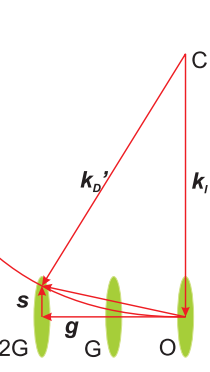
\includegraphics[width=0.3\textwidth]{Figs/Ch2/ewald.png}
	\caption[h] {Intersection of the Ewald sphere centered at C with reciprocal lattice rel-rods. Adapted from \cite{Zhang2008}.}
	\label{2.14}
\end{figure}
\FloatBarrier

Due to the small value of $\lambda$ ( typically picometres), the radius of the Ewald sphere tends to be large relative to the reciprocal lattice spacing, meaning the surface of the sphere is approximately planar relative to the reciprocal lattice rods thus resulting in several spots being observed even in cases where the incident beam is parallel to the zone axis.

\subsubsection{Diffraction Contrast Imaging}
Diffraction contrast imaging is a conventional TEM technique which exploits differing Bragg diffraction conditions in different regions of the sample to create contrast in an image. Image contrast can be obtained either through bright field (BF) \nomenclature[z-BF]{BF}{Bright Field} or dark field (DF) \nomenclature[z-DF]{DF}{Dark Field} imaging, these are shown schematically in Fig \ref{bfdf} below:

\begin{figure}[h]
	\begin{subfigure}[t]{0.5\textwidth}
		\centering
		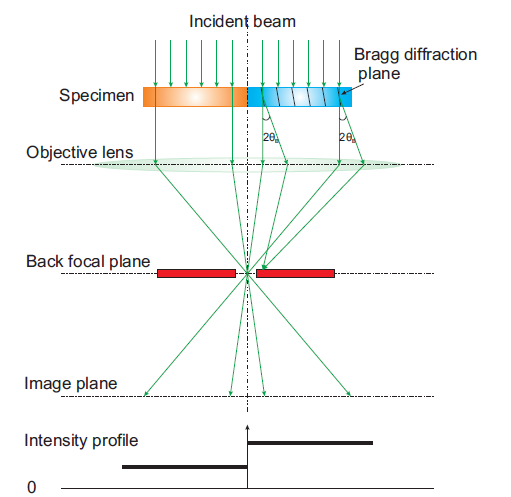
\includegraphics[width = 1\textwidth]{Figs/Ch2/bf.png}
		\caption{}
	\end{subfigure}%
	\hspace*{1cm}
	~	
	\begin{subfigure}[t]{0.44\textwidth}
		\centering
		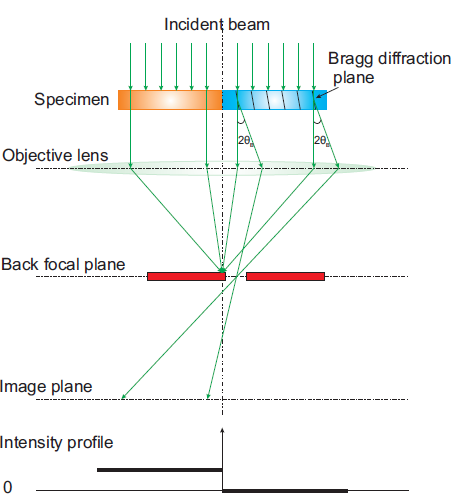
\includegraphics[width=1\textwidth]{Figs/Ch2/df.png}
		\caption{}
	\end{subfigure}
	\caption {a) Bright-field and b) dark-field imaging \cite{Zhang2008}.}
	\label{bfdf}
\end{figure}
\FloatBarrier 

The blue region is shown to satisfy the Bragg diffraction condition for the incident beam whereas the orange region does not. In the case of BF imaging the direct beam is used to generate the image, and as a result the intensity from the orange region is higher than that of the blue region. On the other hand, in DF imaging the diffracted beam is used and the direct beam blocked, resulting in an inverted intensity profile. Barring other electron-specimen interactions such as absorption, the contrast between the BF and DF images is complementary \cite{DavidB.Williams2009}.\\
Figures \ref{bfdf} a) and b) demonstrate that the insertion of an aperture at the back-focal plane (BFP) of the objective lens allows for the selection between BF and DF imaging. Without the objective aperture the image consists of a superposition of BF and DF images with a single DF image for every diffracted beam. In order to ensure the diffracted beam is at the optic axis where spherical aberration of the objective lens is less pronounced the incident beam is often tilted, a practice known as centred dark field (CDF) imaging.
As dislocations in a crystal structure can be found near strained crystal planes, these will result in diffraction contrast in BF or DF images. However it is important to consider that many diffraction spots can be observed in the electron diffraction pattern, which is undesirable for BF or DF contrast imaging. As such the optimal conditions for are defined as the two-beam condition, in which only one set of planes satisfies the Bragg condition \cite{DavidB.Williams2009}, resulting in two beams: the direct beam and the sole diffracted beam. Under the two-beam condition, image contrast is optimized and the intensity of the two beams can be analytically calculated using the Howie-Whelan equations \cite{DavidB.Williams2009} to deliver detailed information concerning the specimen through the interpretation of contrast in the image.

\subsubsection{Weak-Beam Dark-Field Microscopy}

An alternative technique known as weak-beam dark-field (WBDF) \nomenclature[z-WBDF]{WBDF}{Weak-Beam Dark-Field} imaging is often used to image dislocations. As indicated by its name, the technique uses a weakly excited beam to form a DF contrast image. A particular diffraction vector $\mathbf{g}$ associated with a specific set of planes \textit{hkl} is chosen as in regular on-axis DF imaging. The specimen is then tilted to introduce a large excitation error $\mathbf{s_{g}}$ and bring the first diffraction order G onto the optic axis, in doing so the 3G reflection satisfies the Bragg diffraction and appears brighter, whilst the zero-order beam is very weak as shown schematically below:

\begin{figure}[h]
	\begin{subfigure}[t]{0.5\textwidth}
		\centering
		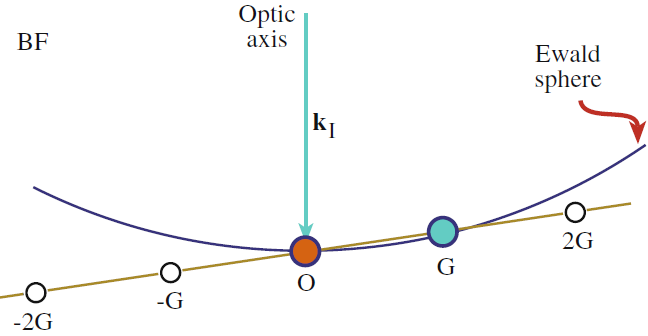
\includegraphics[width = 1\textwidth]{Figs/Ch2/w1.png}
		\caption{}
	\end{subfigure}%
	\hspace*{1cm}
	~	
	\begin{subfigure}[t]{0.44\textwidth}
		\centering
		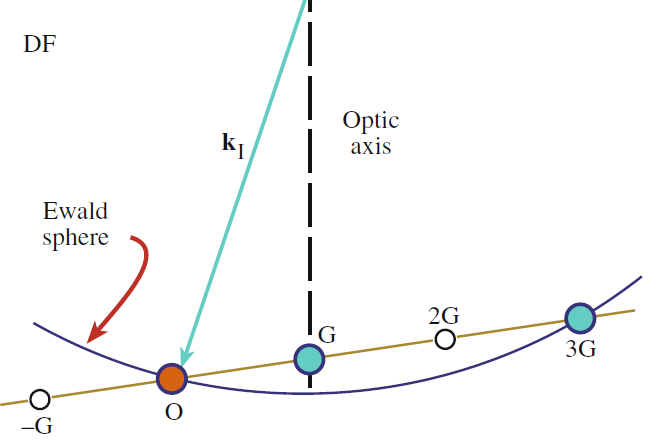
\includegraphics[width=1\textwidth]{Figs/Ch2/w2.png}
		\caption{}
	\end{subfigure}
	\caption {Specimen is tilted from a) to b) for the g-3g condition \cite{DavidB.Williams2009}.}
	\label{wbdf}
\end{figure}
\FloatBarrier 


As such, most of the lattice planes within the specimen are rotated away from the Bragg condition but near the cores of dislocations these are bent back and appear as high intensity features. The high contrast enables highly detailed imaging of dislocations \cite{DavidB.Williams2009}, as shown in Fig.\ref{shellywbdf}.

\begin{figure}[!ht]
	\centering
	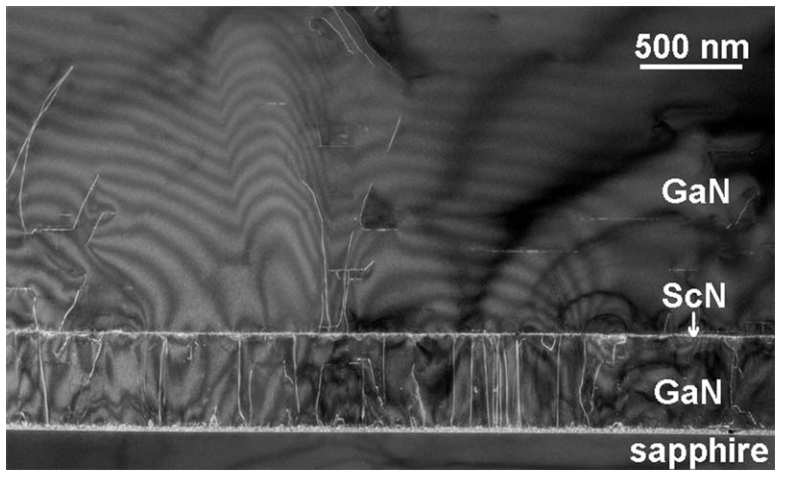
\includegraphics[width=0.7\textwidth]{Figs/Ch2/moramwbdf.png}
	\caption[h] {WBDF imaging of dislocations \cite{Moram2007}.}
	\label{shellywbdf}
\end{figure}
\FloatBarrier



\subsection{Scanning Transmission Electron Microscopy}

Scanning transmission electron microscopy (STEM) differs from conventional TEM in that a converged electron beam is utilised to generate an image as opposed to a parallel incident beam as described in section \ref{TEMconventional}. The convergence of the electron beam generates a probe which can be as small as several angstroms which is focused and scanned across the sample. Each pixel in the image generated by this technique is acquired from the probe in a separate position by collecting radiation emitted from the sample generated by irradiation from the beam.\\
A critical parameter in STEM is the brightness of the source which determines the current in the electron probe. Consequently, field emission guns (FEG) are favoured over thermionic guns such as tungsten or $\mathrm{LaB_{6}}$ for use in STEM. Another factor which contributes to the preference for FEGs in STEM is the increased spatial localisation of the electron emission compared to thermionic sources, which allows for a smaller probe.\\
The probe in STEM is a demagnified image of the crossover from the electron gun. The figure below illustrates how a strong gun lens results in a cross over close to the gun such that fewer electrons travel through the collector aperture, leading to a smaller probe with a lower current on the sample. 

\begin{figure}[!ht]
	\centering
	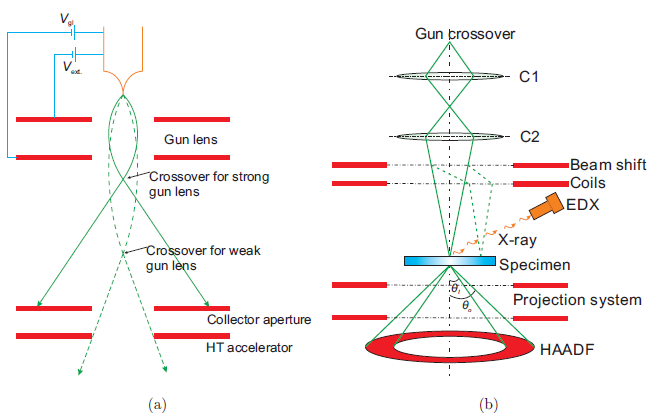
\includegraphics[width=1\textwidth]{Figs/Ch2/STEM}
	\caption[h] {Illustration of a) the FEG source and gun lens b) the column of a STEM with a HAADF for z-contrast imaging and EDX detector \cite{Zhang2008}.}
	\label{STEM}
\end{figure}
\FloatBarrier

As different STEM techniques such as high-angle annular dark-field (STEM-HAADF) imaging, energy dispersive X-ray spectroscopy (STEM-EDX) or convergent beam electron diffraction (STEM-CBED) imaging will require different probes for optimal results, the strength of the gun lens allows for the adjustment of the required parameters \cite{DavidB.Williams2009}.\\
STEM-HAADF is a STEM technique which allows for what is commonly known as Z-contrast imaging, or imaging by atomic number. The basic principle of operation relies on the fact that electrons scattered by atoms at relatively large angles are mostly incoherent and can be considered as particles rather than waves. At high angles, the intensity of the scattered electrons is proportional to the square of the atomic number Z \cite{Howie1979} thus allowing the determination of atomic number of the material at the location of the probe from the brightness of the collected signal. Thus, the use of a high-angle annular dark-field detector allows for the collection of electrons scattered at high angles and the reduction in electrons scattered at low angles, as shown in Fig \ref{STEM} b). The magnification in STEM-HAADF imaging
is controlled by varying the size of the area scanned by the probe, rather than through the use of lenses as in conventional TEM. Strong contrast is typically obtained in HAADF images of III-nitride heterostructures due to the large difference in atomic numbers between the group III elements.

\subsection{Energy-Dispersive X-ray spectroscopy}
Electron-induced X-ray emission allows for the characterisation of sample composition. The high-energy electron beam incident on the sample in TEM can lead to the ionisation of electrons of the inner orbitals, generating vacancies. As electrons from higher energy orbitals relax into this vacancy a characteristic X-ray is released, with an energy equal to the difference between the two states involved in the relaxation transition.\\
Siegbahn notation is used to describe characteristic X-ray lines: the first component is the elemental atom emitting the X-ray, second is the electron shell which was ionized to emit the X-ray ( K, L or M) and the final component describes the relative intensity of the line for each shell (in order of decreasing intensity: $\alpha, \beta, \gamma$) \cite{Facility}. These are shown schematically in Fig.\ref{xray}

\begin{figure}[!ht]
	\centering
	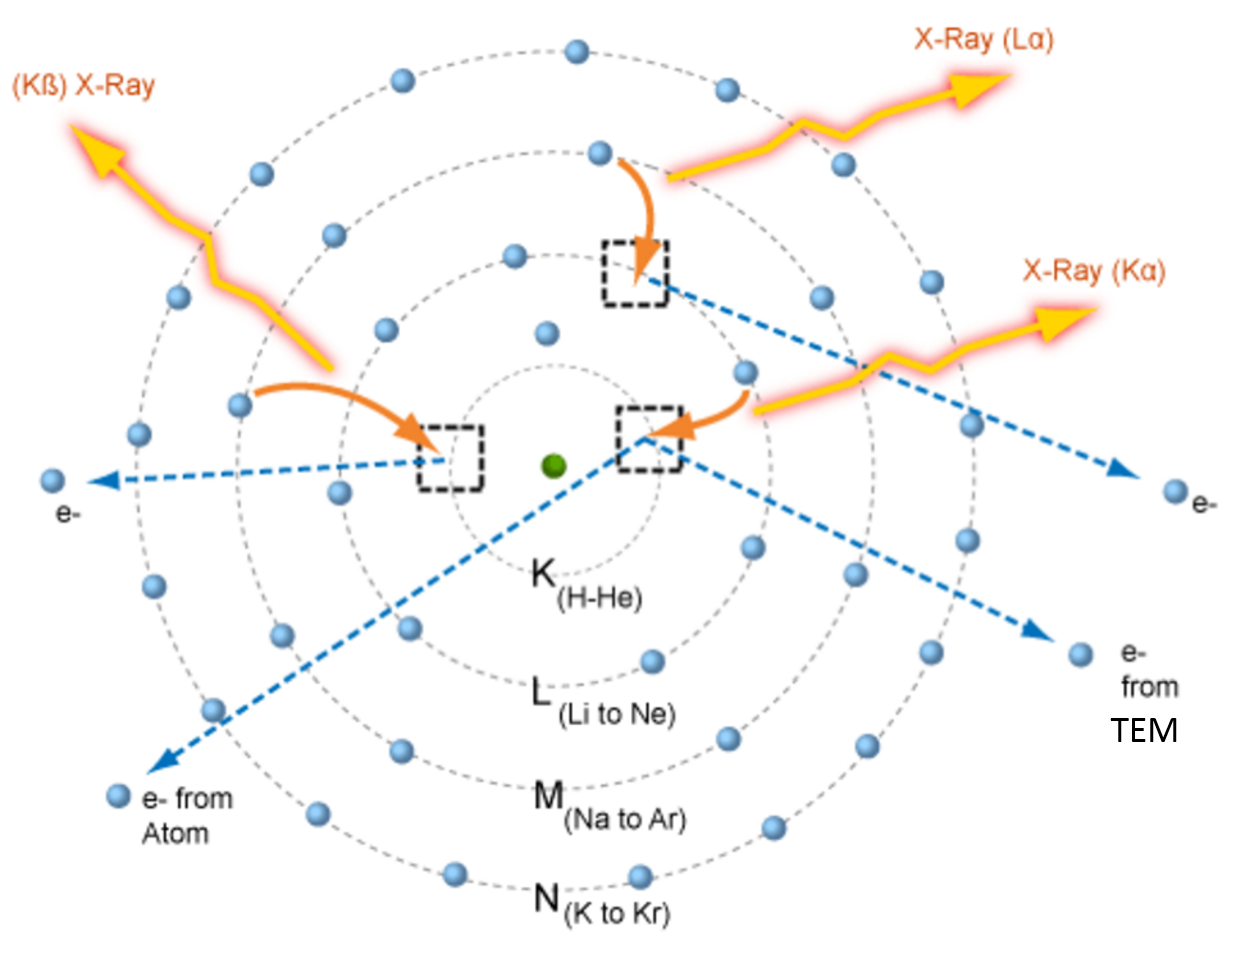
\includegraphics[width=1\textwidth]{Figs/Ch2/xray}
	\caption[h] {$K_{\alpha}, K_{\beta}, and L_{\alpha}$ X-rays and their associated electronic transitions. Adapted from \cite{Facility}}
	\label{xray}
\end{figure}
\FloatBarrier

These characteristic X-rays can be collected using an energy dispersive detector, where the X-rays generate electron-hole pairs in a silicon {\textit p-i-n} junction.\\
Energy-Dispersive X-ray spectroscopy (EDX) is typically used in STEM mode, where the electron beam is condensed into a small probe, which leads to the majority of the X-rays being emitted from a small volume in the sample. This enables the acquisition of spatially resolved elemental maps.

\section{Electron Tomography}
TEM provides a plethora of techniques with which to characterise nano-scale structures, however it is often insufficient to ascertain the 3D morphology of complex structures as it deals with projections of the specimen. A typical exmaple of this is  network of super-imposed particles in which particles overlapping in the projection may not in fact be in contact in real space \cite{Divitni2012}.\\
Tomographic reconstruction is a technique that has been widely used to infer 3D volumes from series of 2D projections. A prime example of this is computed axial tomography scanning (CAT-scanning), a technique that has become prevalent in healthcare. The first demonstration of tomography applied to electron microscopy was reported at the MRC laboratory in Cambridge by De Rosier and Klug \cite{DeRosier1968}. Since then, electron tomography (ET) has progressed in leaps and bounds due to advances in technology pertaining to both microscopy and tomographic reconstruction.\\
The fundamental tenet of tomography lies in the projection theorem developed by Radon at the dawn of the 20th century. The implication of the theorem is that the acquisition of a set of projected images of an object at varying angles can allow for the reconstruction of the full 3D Fourier transform of said object, and consequently the morphology of the object in real space \cite{Divitni2012} as shown in Fig.\ref{Midgley}.a)\\
\begin{figure}[!ht]
	\centering
	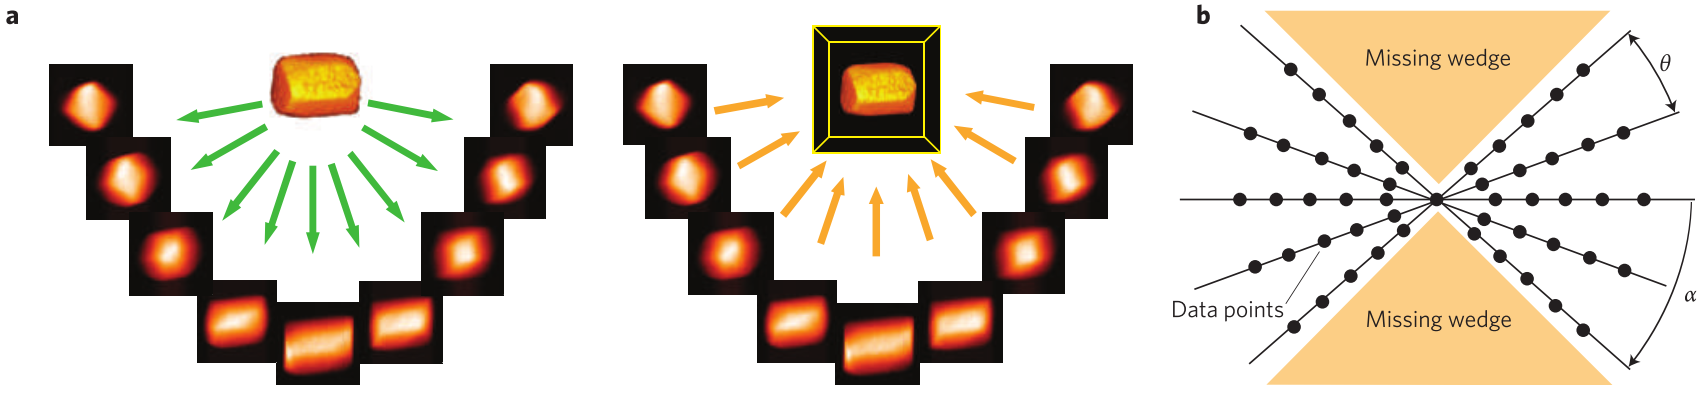
\includegraphics[width=1\textwidth]{Figs/Ch2/tomo}
	\caption[h] {Two-stage tomography process: a tilt series of an object is acquired, then the back projection of these images is used to reconstruct a 3D model of the object \cite{Midgley2009}.}
	\label{Midgley}
\end{figure}
\FloatBarrier

In practical terms, the angular range of the tilt series is an important consideration. A full tilt series acquired between the range $\pm 90^{\circ}$ allows for minimal anisotropy artifacts. However, typical TEM stage and holder combinations will only allow for a range of $\pm 78^{\circ}$ due to the pole-piece gap, leading to a missing wedge of data which results in distortion in the 3D reconstruction \cite{Mobus2007}. Despite these issues, it has been shown that for tilt ranges larger than $\pm 75^{\circ}$, the elongation of features due to the missing wedge is below $10 \%$ and the volume fraction estimate is within experimental error as other factors such as the interval between images in the series and post-processing can also influence the accuracy of the reconstruction \cite{Kawase2007}. \\
In order for the reconstruction to be successful, the signal used in the tilt-series must depend monotically on the thickness of the sample ( or some other physical property) \cite{Frank2006}. In the case of HAADF-STEM imaging, this is true as the signal intensity depends both on specimen thickness and atomic number.	


\section{Atomic Force Microscopy}
Atomic force microscopy  \nomenclature[z-AFM]{AFM}{Atomic Force Microscopy} is a non-destructive characterisation technique which employs a sharp tip mounted on a cantilever which is rastered across a sample surface. Tip-surface interactions result in changes cantilever position which are measured using the reflection of laser light reflecting off the cantilever and a four-quadrant photodetector as shown in Fig.\ref{2.1}.

\begin{figure}[h]
	\centering
	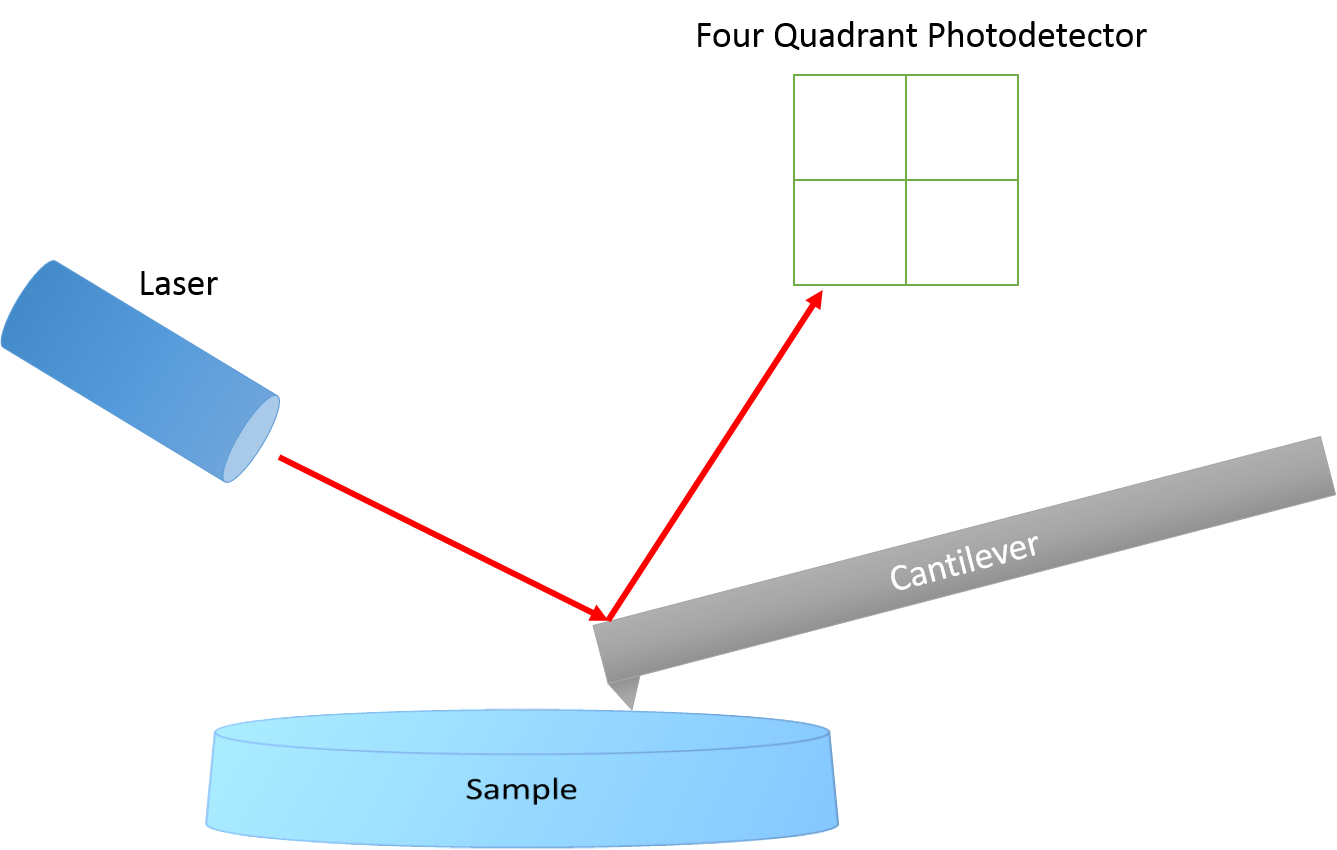
\includegraphics[width=0.7\textwidth]{Figs/Ch2/AFM.png}
	\caption {Schematic of an atomic force microscope.}
	\label{2.1}
\end{figure}
\FloatBarrier

The positioning and movement of the tip is achieved through the use of piezo-electric actuators. In contact mode, a feedback circuit is used to apply a voltage to the piezoelectric crystal in order to maintain a constant tip-sample separation should the tip encounter any features, thus avoiding damage to either the tip or sample. The voltage required to maintain this distance (also known as the setpoint) is registered at each pixel of the scan and is used in conjunction with calibration data to determine a vertical displacement value, thus generating a topographic image.\\
An alternative mode of operation known as tapping mode is often referred to contact mode. In this mode of operation the tip is made to oscillate close to its resonant frequency by the piezocrystal. Contact  between the tip and the sample is achieved at the lowest point of each oscillation, which damps the oscillation of the tip. The oscillation frequency is maintained by the piezoelectric crystal, thus allowing for the generation of a topographic map. Tapping mode is often preferred to contact mode due to the exclusion of lateral friction which can cause tip wear and sample damage.\\
The forces experienced by the tip vary depending on the tip-sample separation, as shown in Fig.\ref{2.2}. Van der Walls forces dominate at large separations attractive the tip to the surface. As the distance is reduced repulsive forces such as hard-sphere repulsion, electron-electron Coulomb interaction and the Pauli-exclusion interaction begin to dominate. The sum of these forces result in cantilever deflection, changing the tip-sample interaction.

\begin{figure}[h]
	\centering
	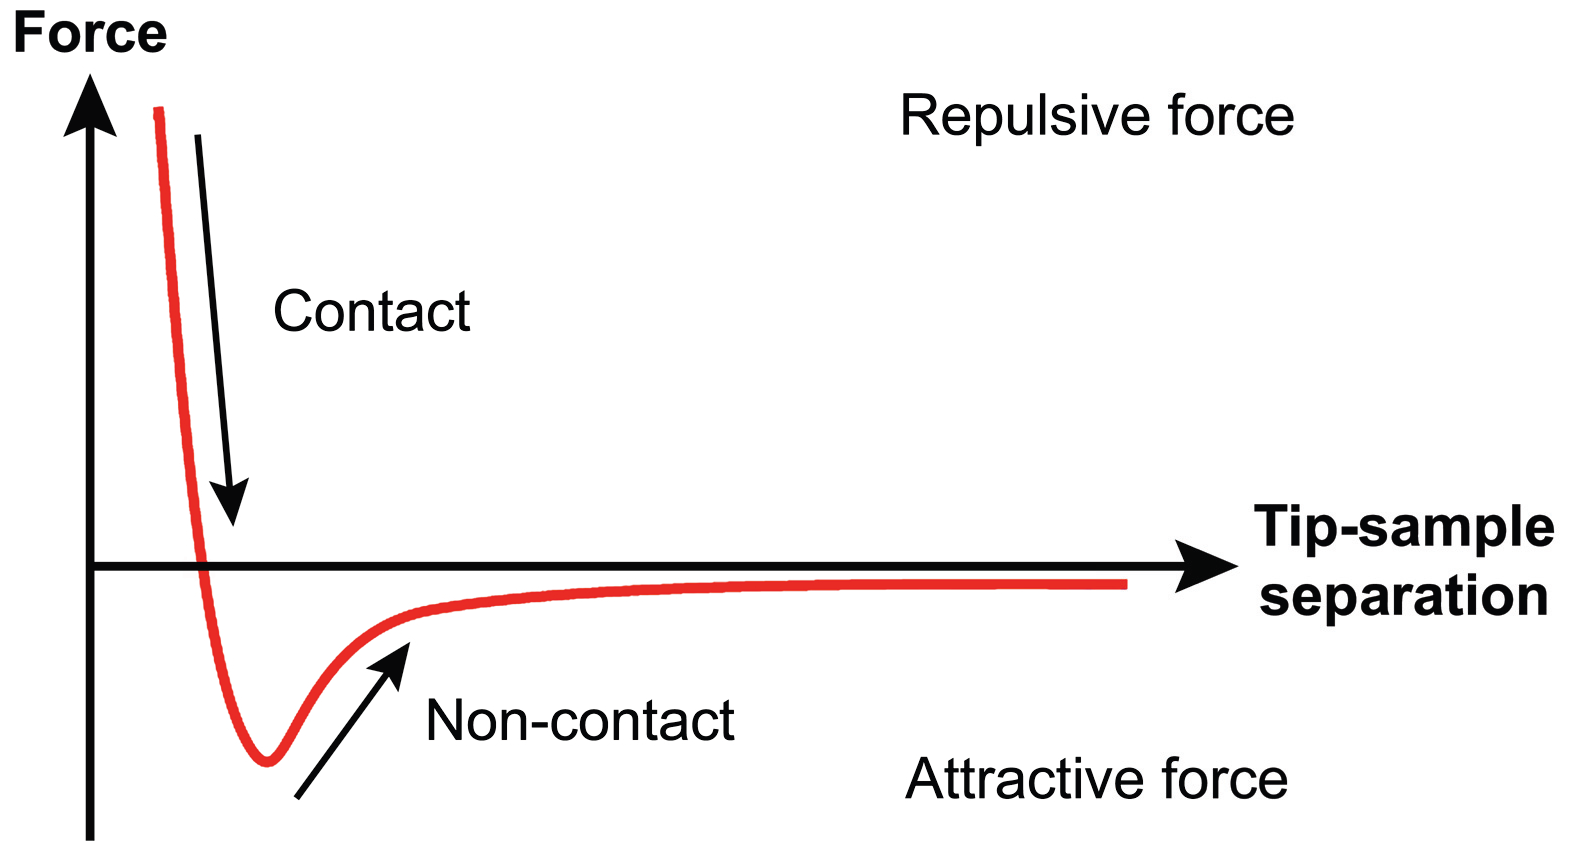
\includegraphics[width=0.7\textwidth]{Figs/Ch2/AFMint.png}
	\caption {The effect of separation on the tip-sample interaction force \cite{Zhu2010}.}
	\label{2.2}
\end{figure}
\FloatBarrier

AFM offers excellent vertical resolution limited only by the probes vertical movement and external noise. However, the lateral resolution of this technique is heavily dependent on the shape and size of the tip employed. This is highlighted by Fig.\ref{2.3} which depicts a hemispherical tip scanning across a flat-topped island. The apex of the tip is in contact with the surface, but the side of the island also experiences some contact: in this case there is a distinction between the two cases shown in Fig.\ref{2.2}a) and b) as the error in the measured width of the island varies based on the relative size of the measured object to the tip.

\begin{figure}[h]
	\begin{subfigure}[t]{0.4\textwidth}
		\centering
		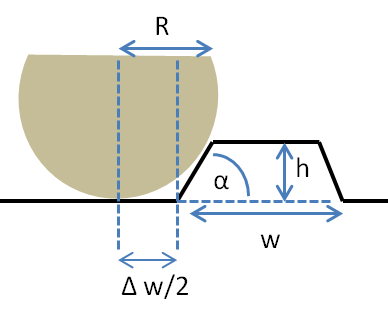
\includegraphics[width = 1\textwidth]{Figs/Ch2/afm1.png}
		\caption{}
	\end{subfigure}%
	\hspace*{1cm}
	~	
	\begin{subfigure}[t]{0.4\textwidth}
		\centering
		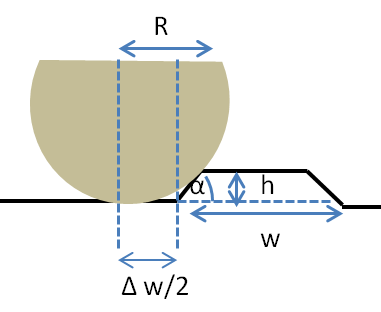
\includegraphics[width=1\textwidth]{Figs/Ch2/afm2.png}
		\caption{}
	\end{subfigure}
	\caption {Interaction of a hemisphere with a flat-topped island for the cases a) $h > R(1-cos(\alpha))$ and b) $h < R(1-cos(\alpha))$ adapted from \cite{Oliver2008}. }
	\label{2.3}
\end{figure}
\FloatBarrier 

Similarly, when measuring depth rather than height the ability of the tip to penetrate into the spaces being measured is also a crucial consideration, as shown in Fig.\ref{2.4}. Thus, increasing the gradient of the tip and minimizing the tip apex are desirable to reduce tip-related measurement artefacts when performing atomic force microscopy.

\begin{figure}[h]
	\centering
	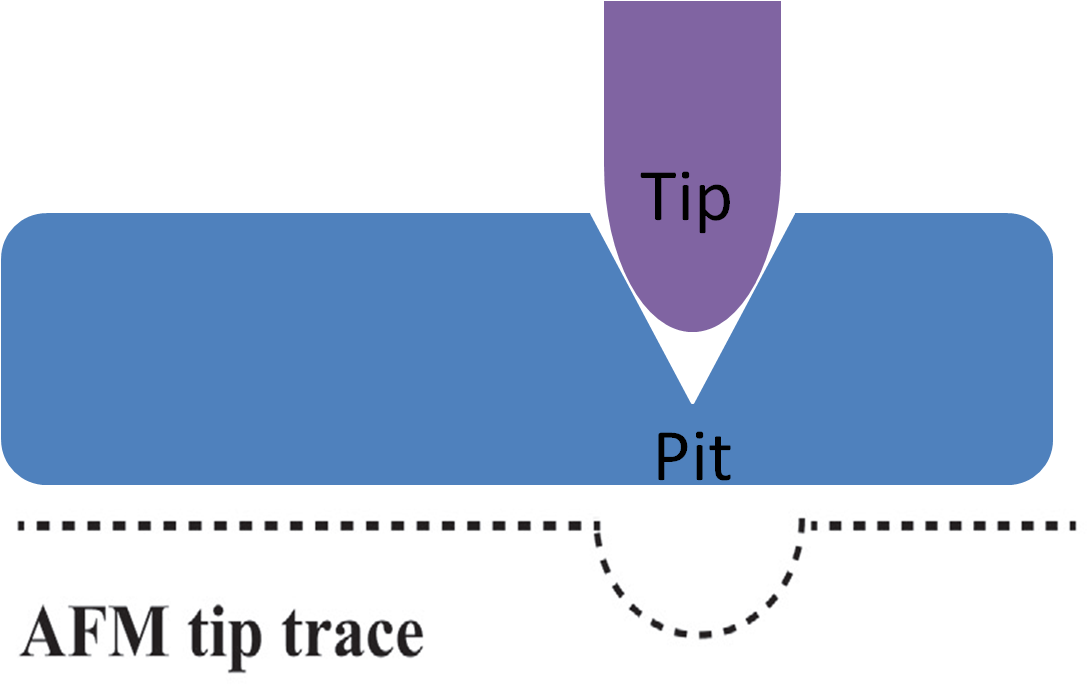
\includegraphics[width=0.4\textwidth]{Figs/Ch2/afm3.png}
	\caption {Measurement error in the depth of a pit caused by the finite width of the AFM tip.}
\end{figure}
\FloatBarrier

\subsubsection{Conductive Atomic Force Microcsopy}

Conductive atomic force microscopy \nomenclature[z-C-AFM]{C-AFM}{Conductive Atomic Force Microscopy} is a technique which combines AFM with local conductivity measurements. In order to perform C-AFM a conductive probe tip is brought close to contact with the sample and a bias is applied between the tip and the sample. The short tip-sample separation causes electron wavefunctions in the tip and sample to overlap, thus allowing a tunneling current to be generated through the application of a bias. C-AFM thus allows for the simultaneous measurement of tip-sample current flow and surface morphology, making it an extremely powerful tool to probe local sample conductivity. 


% Uncomment this line, when you have siunitx package loaded.
%The SI Units for dynamic viscosity is \si{\newton\second\per\metre\squared}.


\section{Scanning Electron Microscopy Techniques}

A scanning electron microscope  \nomenclature[z-SEM]{SEM}{Scanning Electron Microscope} (SEM) employs the use of electrons to characterise material morphology and composition. A schematic of a typical SEM design is shown in Fig.\ref{2.4}.

\begin{figure}[h]
	\centering
	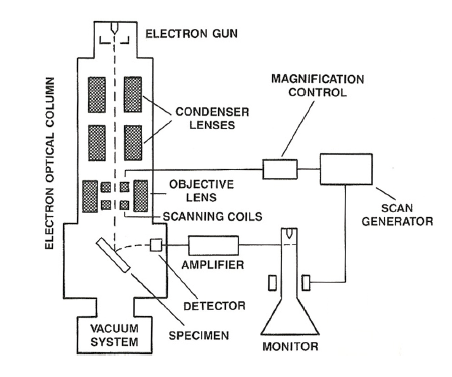
\includegraphics[width=0.6\textwidth]{Figs/Ch2/SEM.png}
	\caption {SEM design \cite{YacobiHolt1990}.}
	\label{2.4}
\end{figure}
\FloatBarrier

The electron gun generates a beam of electrons, typically of energy up to 30 keV. The condenser lenses situated below the gun serve to determine the probe size by adjusting the demagnification of the beam. The objective lens serves to further adjust this demagnification, and is situated directly above the specimen. The scanning coils raster the electron probe across the sample, and the detector thus builds an image of the specimen by collecting various signals which occur due to the electron-specimen interactions.\\
As the beam of electrons interacts with the specimen, various processes occur which generate characteristic signals, as shown in Fig.\ref{2.5} and previously discussed in Section \ref{TEM}. The volume within the sample which contains the energy deposited by the electron beam is known as the interaction volume, the shape and size of which is determined by both the beam energy and sample composition. Inelastic scattering of the electrons results in the production of signals such as secondary electrons \nomenclature[z-SE]{SE}{Secondary Electron} (SEs), Auger electrons and characteristic X-rays. Typically, it is the SEs which are used for imaging in SEMs. Elastic scattering can generate back scattered electrons \nomenclature[z-BSE]{BSE}{ Back Scattered Electron} (BSEs), which are collected through the surface on which the beam is incident. Due to the nature of elastic scattering, BSEs have a strong dependence on atomic, and are can thus be used to produce composition-dependent image contrast.

\begin{figure}[h]
	\centering
	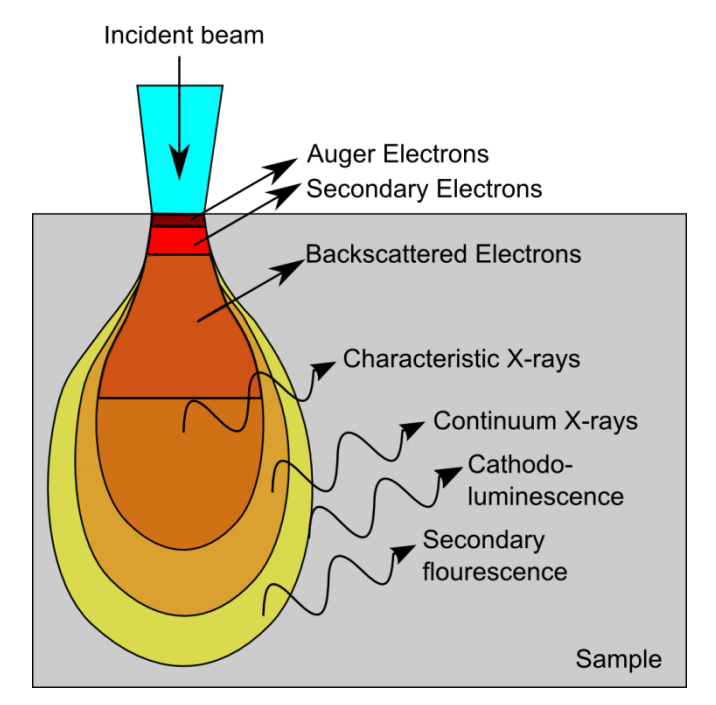
\includegraphics[width=0.6\textwidth]{Figs/Ch2/int.png}
	\caption {Interaction volumes for different interactions of an electron beam \cite{Puchtler2014}.}
	\label{2.5}
\end{figure}
\FloatBarrier



\subsubsection{Cathodoluminescence}

The absorption of primary electrons in a semiconductor can generate electronic excitations, or electron-hole pairs, with light emission occurring as a consequence of their recombination. This process is known as cathodoluminescence \nomenclature[z-CL]{CL}{Cathodoluminescence}(CL). The electronic transitions which are associated with CL emission require lower energies than those needed to excite X-rays.\\
\indent One of the principal advantages of CL in comparison with photo-excitation spectroscopy techniques used on semiconductors is the limitation of the spatial resolution of the technique by the interaction volume of the elecctron beam in the material rather than diffraction, which can be considered an intrinsic limitation of most optical far-field techniques \cite{Edwards2011}. As a result, nanometre-scale characterization of materials can be achieved.\\
\indent Due to the large number of electron-hole pairs generated within the interaction volume of the impinging electron beam on a bulk semiconductor material,all possible transitions within the material tend to be excited, resulting in the crucial limitation of being unable to selectively excite transitions below a certain energy \cite{Edwards2011}. Nonetheless, the versatility of CL as a technique has been amply demonstrated in its ability to shed light on the composition of compound materials such as InGaN/GaN structures \cite{Martin2004}, carrier diffusion length and surface recombination rates \cite{Sercel1989} and even minority carrier lifetimes \cite{YacobiHolt1990}.\\
\indent A schematic view of a set-up for CL imaging is show in Fig.\ref{2.6}:

\begin{figure}[!ht]
	\centering
	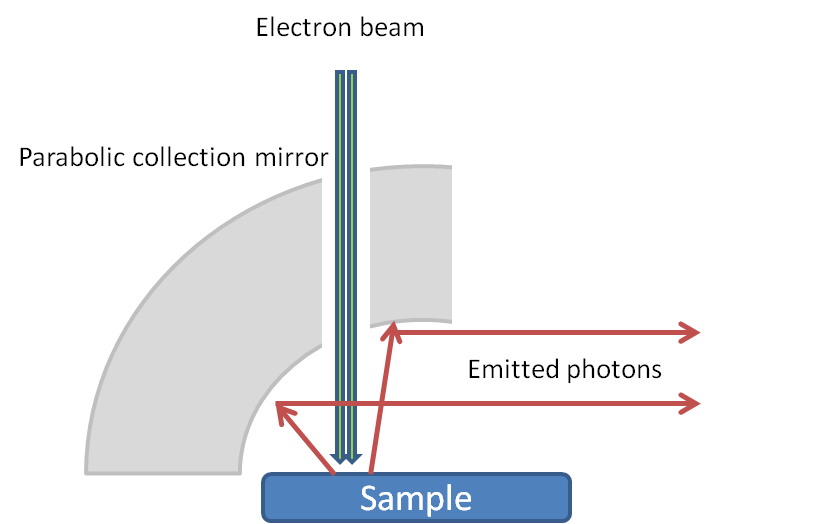
\includegraphics[width=0.5\textwidth]{Figs/Ch2/CL.png}
	\caption[h] {Schematic layout of a CL imaging system.}
	\label{2.6}
\end{figure}
\FloatBarrier

The electron beam is incident on the sample in the SEM chamber and results in the generation of photons which are collected by a parabolic mirror through a high vacuum feedthrough and coupled into a monochromator. Photomultiplier tubes (PMTs) are the most commonly used detector for this set-up. \\
The most basic form of CL imaging is known as panchromatic imaging. In this case, the collected light in its entirety is directed to a single detector and the resulting greyscale image intensity is the product of the spectral response of the system and the emission spectrum \cite{Edwards2011}. An extension of this is the monochromatic imaging mode, in which case only a single band of wavelengths is imaged using a band-pass filter or spectrometer \cite{Edwards2011}.\\
CL hyperspectral imaging, or CL wavelength imaging is an extension of the aforementioned technique whereby a full luminescence spectrum is recorded at each point during a beam scan, enabling the construction of a spatially and spectrally resolved data set.\\
 In the set-up shown in Fig \ref{2.6}, a semi-paraboloidal mirror allows emitted photons to be collected over close to the entire hemisphere. In this case, the beam is scanned across the sample in order to achieve CL hyperspectral imaging, however a number of drawbacks are inherent to this collection geometry:\\
\\\indent - The position of the mirror requires a large working distance and can obscure the optical element thus compromising the imaging capabilities of the microscope.\\
\\\indent - The small distance between the sample and mirror imposes a restriction on the extent to which the sample can be tilted, which can be an issue in the examination of three-dimensional structures.\\
\\\indent - The {\it\'{e}tendue} of the system imposes a strict compromise between the field of view of the microscope and the collection efficiency at the spectrometer \cite{Edwards2011}.\\
\\\indent In an effort to overcome these limitations, CL hyperspectral imaging systems have been developed, whereby light collection is achieved using an objective placed perpendicular to the electron beam as shown below in Fig \ref{2.7}. By allowing the optics to be placed further away from the sample, a far shorter working distance can be used, allowing the electron spot to remain small at low accelerating voltages \cite{Edwards2011}. 

\begin{figure}[!ht]
	\centering
	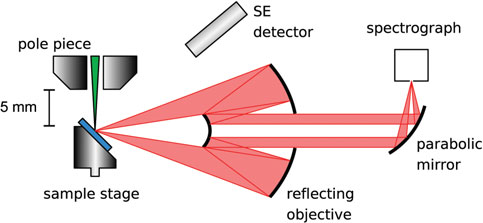
\includegraphics[width=0.5\textwidth]{Figs/Ch2/hyper.png}
	\caption[h] {Schematic layout of a CL hyperspectral imaging system \cite{Edwards2012}.}
	\label{2.7}
\end{figure}
\FloatBarrier

The CL data in this thesis was collected on two separate systems, one employing the collection geometry described in Fig.\ref{2.6} and the other shown in Fig.\ref{2.7}
\subsubsection{Electron-Beam Induced Current}

Electron beam induced current \nomenclature[z-EBIC]{EBIC}{Electron-Beam Induced Current} (EBIC) imaging is a technique complementary to scanning electron microscopy. The premise of the measurement is that minority carriers which arise from the incident electron beam of an SEM on a semiconductor junction can diffuse to the junction where they are separated by the built-in field and collected as current by an external circuit (the EBIC amplifier).\\
Due to the small interaction volumes achievable, EBIC can provide detailed spatial information on minority carrier dynamics. Regions of high signal indicate high collection efficiency and low recombination, for example: the depletion region of a p-n junction appears bright in EBIC imaging. As such EBIC imaging has proven extremely useful in characterising the recombination properties of individual defects across a wide range of semiconductors \cite{Yakimov2002}.  


\section{Hyperspectral Electroluminescence Mapping}
Hyperspectral electroluminescence  \nomenclature[z-EL]{EL}{Electroluminescence} (EL) mapping can be used to characterise local variations in EL in optoelectronic devices. The EL mapping data in this thesis was acquired on a modified electron probe micro-analyser \nomenclature[z-EPMA]{EPMA}{Electron Probe Micro-Analyser} (EPMA). The EPMA consists of a CL system, and can also be used for CL spectroscopy. In order to perform EL mapping, the electron beam is switched off and a pinhole inserted. A forward bias is then applied to the device being characterised and the stage is moved in order to build up a map of EL emission of the device which is collected by a CCD camera to build up a hyperspectral data set consisting of a full spectrum for each pixel.


\section{Dual Beam FIB-SEM}

In this work a dual beam focused ion beam/scanning electron microscope  \nomenclature[z-FIB/SEM]{FIB/SEM}{Focussed Ion Beam/Scanning Electron Microscope} was used to perform sample preparation as well as 'slice and view' tomography experiments. As we have introduced the basic principles behind SEM we will focus on the FIB in this section.
\\ The FIB is an extremely versatile combination of a scanning ion microscope ( similar in principle to the SEM but utilising ions rather than electrons) and a precision machining tool. The ions utilised by the FIB are typically $\mathrm{Ga^{+}}$, though helium sources also exist. A liquid-metal ion source is used to produce the gallium ions which are focused into a beam and onto the surface of a sample in a similar manner to the SEM using electrostatic lenses and apertures. Due to the complementary nature of FIB and SEM instruments, dual beam FIB/SEM machines have been produced in which the techniques are used synergistically to overcome limitations on individual systems. Aside from a standard electron beam, the FIB-SEM contains an additional gallium ion beam at an angle of $\mathrm{52^{o}}$ to the axis of the electron beam as shown in Fig.\ref{2.8}

\begin{figure}[!ht]
	\centering
	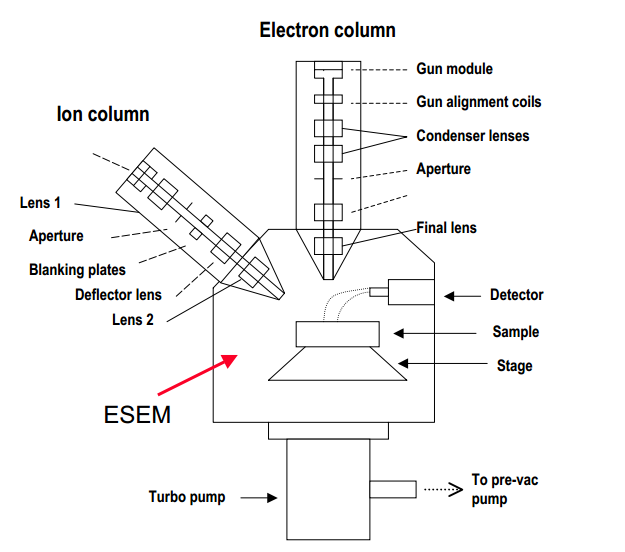
\includegraphics[width=0.6\textwidth]{Figs/Ch2/FIB.png}
	\caption[h] {Diagram of a dualbeam FIB-SEM}
	\label{2.8}
\end{figure}
\FloatBarrier

Due to the large mass of the $\mathrm{Ga^{+}}$ ions relative to electrons the interaction of the focused ion beam with a sample can cause sputtering of the material, thus allowing for the precise removal of material. Often the SEM is used to monitor the milling process of the FIB as electrons cause negligible damage to the sample relative to the ion beam. Beyond the removal of material, the ion beam can also often be used to deposit material. A gas injection system \nomenclature[z-GIS]{GIS}{Gas Injection System} is typically used to achieve this: a gas containing a metal-organic compound is injected into the chamber where it interacts with the targeted ion-beam  at the surface of the sample leading to the heavier metal atoms remaining at the sample surface whilst the organic material is evacuated by the chamber vacuum system. Typically, platinum or carbon can be deposited using this method, though the platinum often contains carbon and other impurities rendering effectively semi-insulting. 

\subsection{Sample Preparation}
Transmission electron microscopy \nomenclature[z-TEM]{TEM}{Transmission Electron Microscopy} requires electron transparent samples, typically of a thickness on the order of 100-150nm. As such the dual beam FIB/SEM allows for site-specific TEM specimen preparation. Unless otherwise stated, all the TEM samples prepared in this work were produced using the FIB/SEM.\\
The specimen preparation method is shown in Fig.\ref{2.9} is as follows:\\
\indent - A region of interest on the sample surface is identified.\\
\indent - A protective layer of metal is deposited using the GIS system, first with the electron beam then with the ion beam.\\
\indent - Ion milling is used to form trenches on either side of the deposited protective layer\\
\indent - A probe is then attached to the lamella by connecting the two with ion-beam deposited metal and used to lift the lamella out.\\
\indent - The lamella is then transferred to a TEM grid, where it is thinned to a suitable thickness.


\begin{figure}
	\begin{subfigure}[b]{0.3\textwidth}
		\centering
		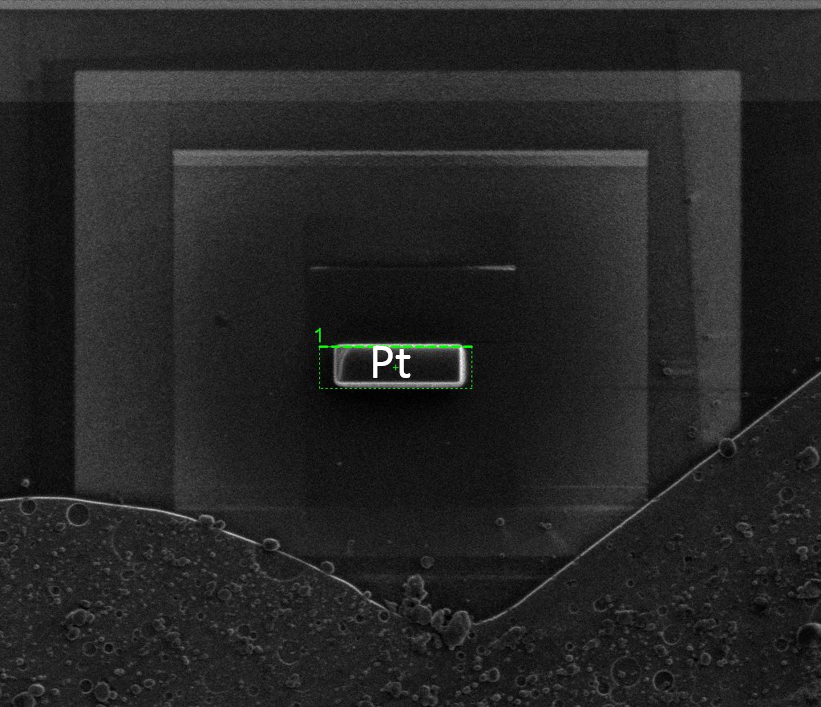
\includegraphics[width=.95\linewidth]{Figs/Ch2/FIB1}
		\caption{}
		
	\end{subfigure}%
	\hspace*{0.5cm}
	\begin{subfigure}[b]{0.3\textwidth}
		\centering
		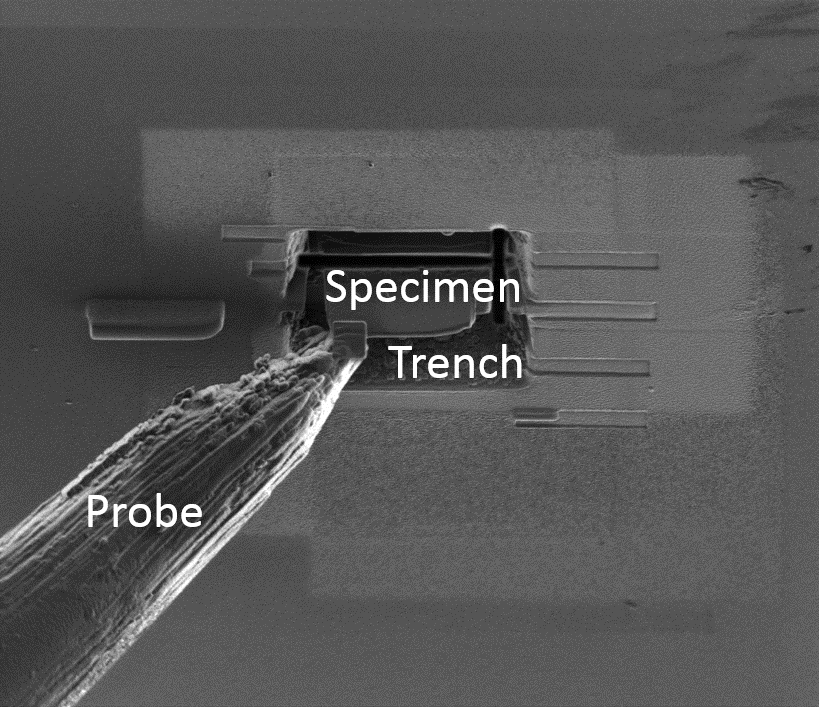
\includegraphics[width=.95\linewidth]{Figs/Ch2/FIB2}
		\caption{}
		
	\end{subfigure}%
	\hspace*{0.5cm}
	\begin{subfigure}[b]{0.3\textwidth}
		\centering
		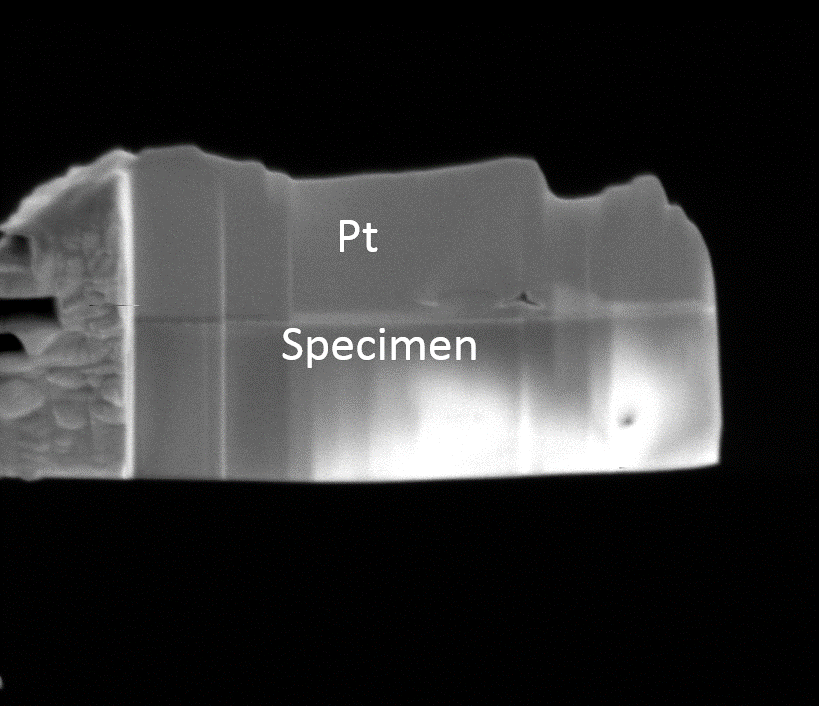
\includegraphics[width=.95\linewidth]{Figs/Ch2/FIB3}
		\caption{}
	\end{subfigure}%
	
	\caption{FIB/SEM lamella lift-out and polishing process: a) Protective Pt layer deposition, b) trench milling and Lamella lift out c) final thinning.}
	\label{2.9}
\end{figure}

\FloatBarrier

\subsection{Tomography}
FIB/SEM tomography, often referred to as 'slice and view', is a technique which has become relatively widespread in materials and life sciences due to the variety of detection modes available in commercial systems as well as the resolution and volume of material which can be analysed. Typical resolutions that can be achieved ( voxel sizes) are in the range 5-10 nm.\\
In FIB/SEM tomography, a small volume of the sample is selected for analysis. This volume is then typically coated with a layer of protective metal in order to prevent ion beam damage. Serial sectioning is then used to analyse the sample: alternating turns of milling and imaging allow for the sequential erosion of thin layers of material and subsequent imaging as shown in Fig.\ref{2.10}. In this work we employ only the use of the SE detector for imaging.

\begin{figure}[!ht]
	\centering
	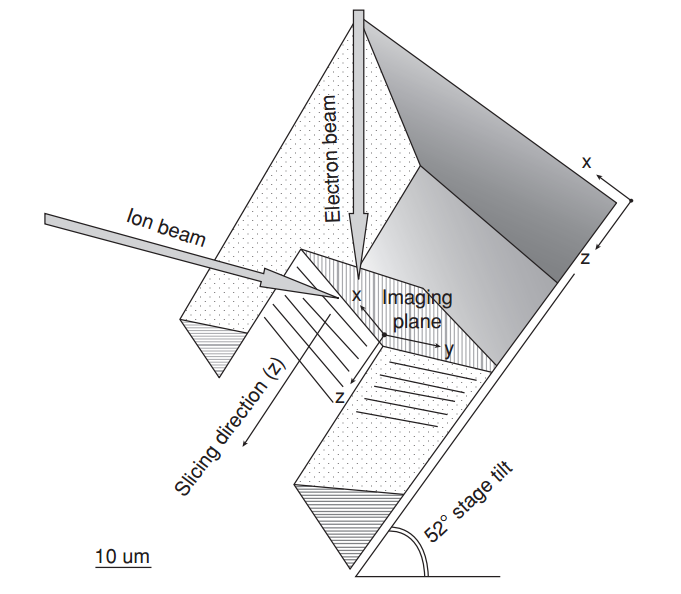
\includegraphics[width=0.9\textwidth]{Figs/Ch2/SnV.png}
	\caption[h] {Schematic of sample geometry for serial sectioning in a FIB/SEM instrument \cite{Holzer2004}.}
	\label{2.10}
\end{figure}
\FloatBarrier

The purpose of serial sectioning is to produce a stack of images which can be transformed into a voxel-based volume data set. As such the thickness of the milled layers should match approximately with the resolution in the imaging plane.\\
Perhaps the most challenging task in FIB/SEM tomography lies in the extraction of information from the reconstructed 3-D image volume. This procedure, known as 'stack-processing', is very similar to reconstruction protocol used for electron tomography and can be described as follows:\\
\indent - 3-D volume reconstruction by stack alignment.\\
\indent - Image defect correction ( noise reduction etc...)\\
\indent - Segmentation and recognition of objects.\\
\indent - Visualization of voxel-based volume data.\\
\indent - Quantitative analysis of features.





